\documentclass{article}

%% Denote paragraphs with vertical space rather than indenting (not critical)
\usepackage{parskip}

%% Support for URL in introductory text (not needed for main example)
\usepackage{url}

%% *** Enable PGFPLOTS (automatically enables TikZ) ***
\usepackage{pgfplots}

%% Prevent some PGFPLOTS messages (not critical)
\pgfplotsset{compat=1.18,compat/show suggested version=false}

%% *** For advanced table manipulations ***
\usepackage{pgfplotstable}


\begin{document}

%% Introductory Text
Example 8.3 from the book\\
\emph{Unlocking LaTeX Graphics: A Concise Guide to Ti$k$Z/PGF and PGFPLOTS}.\\
For more information, visit \url{https://latex-graphics.com}.
\par\bigskip

%% *** START OF EXAMPLE CODE ***
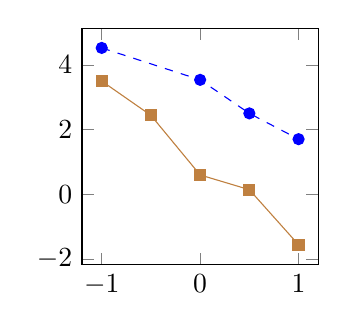
\begin{tikzpicture}
  \pgfplotstableread[col sep=comma]{x, f1, f2
    -1.000000,4.525804,3.499907
    -0.500000,NaN,2.439197
    0.000000,3.537790,0.595883
    0.500000,2.500406,0.139694
    1.000000,1.702716, -1.563586
  }{\mydata}
  \begin{axis}[scale only axis,width=3cm, height=3cm]
    \addplot[blue,dashed,mark=*,every mark/.append style={solid}] table{\mydata};
    \addplot[brown,mark=square*] table[y=f2]{\mydata};
  \end{axis}
\end{tikzpicture}
%% *** END OF EXAMPLE CODE ***

\end{document}
